\documentclass{beamer}
\usepackage{algorithm}
\usepackage{algpseudocode}
\usepackage{amsmath}
\usepackage{hyperref}
\usetheme{Antibes}

\hypersetup{pdfstartview={Fit}}
\title{trAIner}
\subtitle{An immersive artificial intelligence game for everybody!}

\author{\textbf{Lucas Mahler, Patrick Gautheret, Kasparas Gudzius, Rahul Tak, Oleksandr Shlapak}}
\institute{University of Applied Sciences Ulm}
\date{\today}

\begin{document}

\begin{frame}
\titlepage
\end{frame}
\section{Introduction}
\begin{frame}
    \frametitle{Motivation}
    \large
    \textit{"We were supposed to make AI do all the work and we play games but we do all the work and the AI is playing games!"}\newline\\
    -Andrey Karpathy
\end{frame}
\begin{frame}
    \frametitle{Outline}
    \tableofcontents
\end{frame}
\section{User Pitch}
\begin{frame}
    \frametitle{What is trAIner?}
    A single, cross platform game experience:
    \begin{itemize}
        \item Implementing the concept of Artificial Intelligence in a Java based application.
        \item trAIner is an absorbing, immersive game experience
        \item Lets the player develop and train their own AI 
        \item Lets the user build his own maps
    \end{itemize}

\end{frame}
\begin{frame}
    \frametitle{Members:}
    On Github: github.com/tr-AI-ner/trAIner
\begin{itemize}
        \item Patrick Gautheret: ElectrifyPowr
        \item Lucas Mahler: Lugges991
        \item Kasparas Gudzius: kasparasGud
        \item Rahul Tak: takrahul
        \item Oleksandr Shlapak: oleksandrshlapak
    \end{itemize}

\end{frame}

\subsection{Audience}
\begin{frame}
    \frametitle{Targeted Audience}
    \begin{itemize}
        \item Gaming Lovers
        \item Tech Enthusiasts
        \item AI Geeks
    \end{itemize}
\end{frame}

\subsection{Features}
\begin{frame}
    \frametitle{3 Different Modes:}
    \large
    \begin{itemize}
        \item Play the Game!
        \item Build Your Own Maps!
        \item Let the AI Play!
    \end{itemize}
\end{frame}

\subsection{Functionality}
\begin{frame}
    \frametitle{Tools and Technology}
   \large
    \begin{itemize}
        \item Java 
        \item Genetic Algorithms
        \item Local Storage
    \end{itemize}

\end{frame}

\begin{frame}
    \frametitle{Builder Mode:}    
    \begin{itemize}
        \item Place/Delete building blocks
        \item Make use of enemies with different behavior
        \item Save \& Load your own creations
    \end{itemize}
\end{frame}
\begin{frame}
    \frametitle{Player Mode:}    
    \begin{itemize}
        \item Play the default
        \item Play on your own maps
        \item Test your might on the challenges
    \end{itemize}
\end{frame}


\begin{frame}
    \frametitle{Use Cases}
    \begin{figure}
        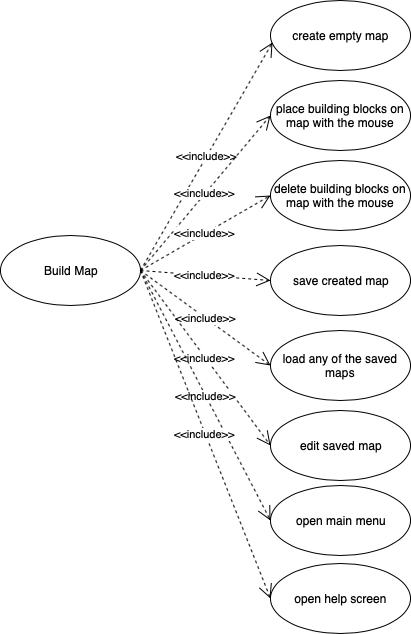
\includegraphics[scale=0.25]{resources/Use_Case_Build_Map.png}

    \end{figure}

\end{frame}
 
\begin{frame}
    \frametitle{Use Cases}
    \begin{figure}
        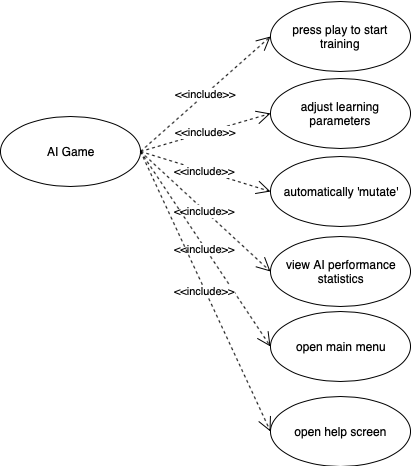
\includegraphics[scale=0.37]{resources/Use_Case_AI_Game.png}

    \end{figure}

\end{frame}


\begin{frame}
    \frametitle{Use Cases}
    \begin{figure}
        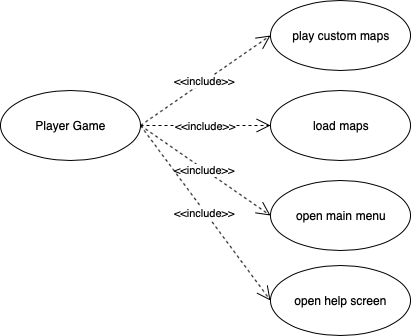
\includegraphics[scale=0.5]{resources/Use_Case_Player_Game.png}

    \end{figure}

\end{frame}

\subsection{Genetic Algorithm}
\begin{frame}
    \frametitle{Genetic Algorithm}

    \begin{itemize}
        \item Darwin as inspiration
        \item Natural concepts of survival of the fittest
        \item Implementation of selection, crossover and mutation
    \end{itemize}

\end{frame}

\begin{frame}
    \frametitle{How Does the GA Work?}
    \begin{figure}
        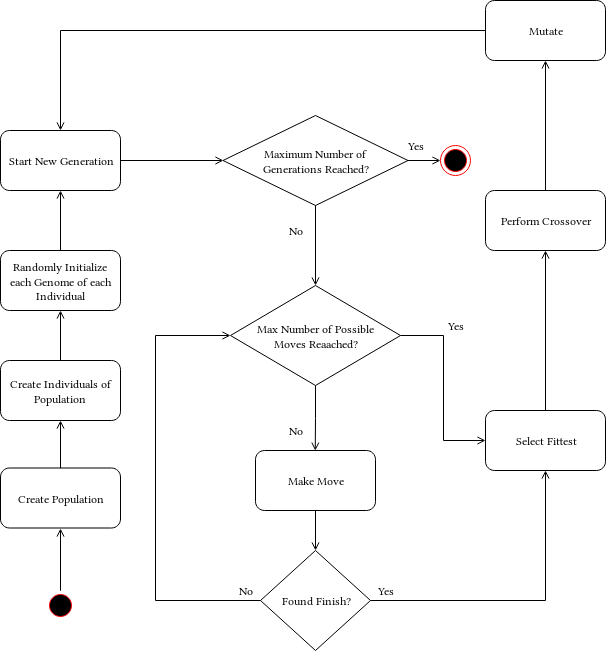
\includegraphics[scale=0.3]{resources/GeneticAlgorithm.png}

    \end{figure}

\end{frame}

\section{Investor Pitch}
\subsection{Requirements}
\begin{frame}
    \frametitle{Functional \& Non-Functional Requirements}
    \begin{figure}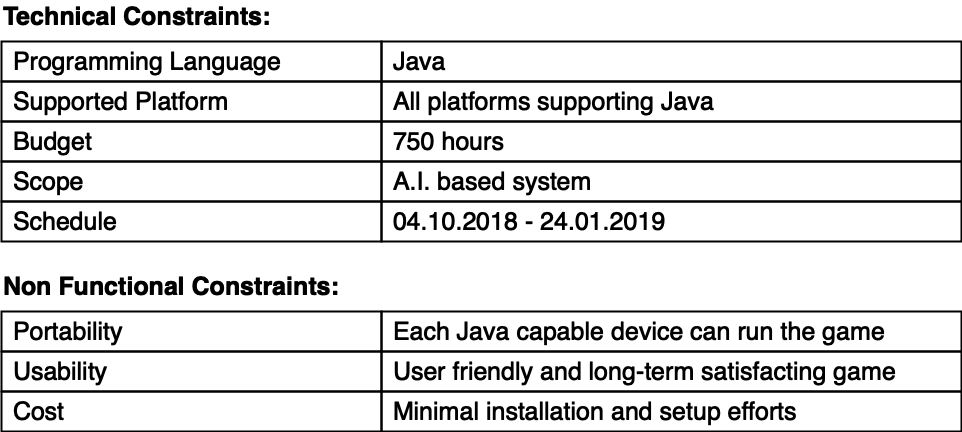
\includegraphics[scale=0.3]{resources/Software_requirements_table_bb.png} 

    \end{figure}
\end{frame}


\subsection{Architectural Patterns}
\begin{frame}
    \frametitle{Architectural Patterns Used:}
    \begin{itemize}
        \item Game Loop
        \item Type Object
        \item Double Buffer
    \end{itemize}

\end{frame}

\begin{frame}
    \frametitle{Game Loop}
    \begin{figure}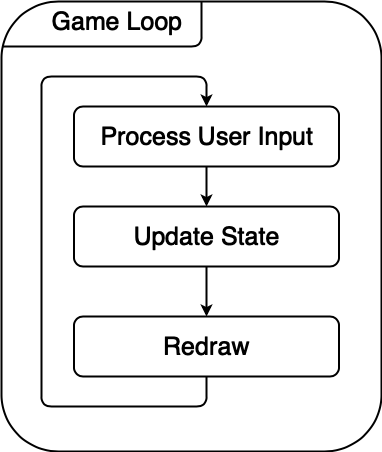
\includegraphics[scale=0.4]{resources/Game_loop_flow_diagram_bb.png} 

    \end{figure}

\end{frame}

\begin{frame}
    \frametitle{Type Object}
    \begin{figure}
        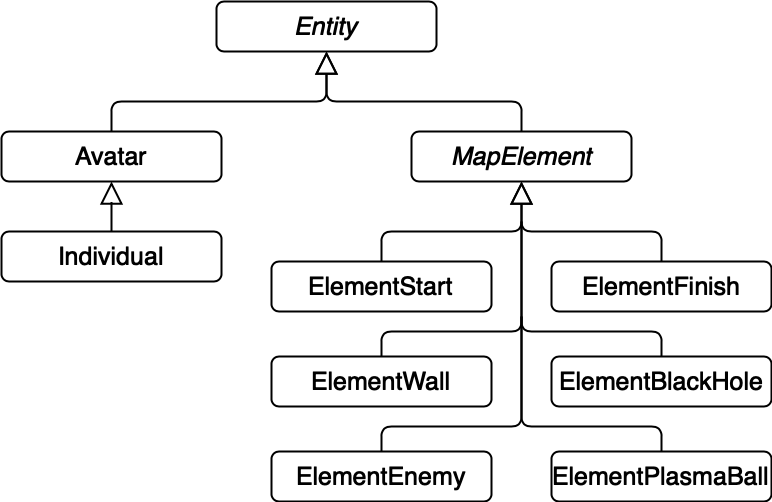
\includegraphics[scale=0.3]{resources/Typed_Objects_Diagram_Entity_bb.png} 

    \end{figure}

\end{frame}


\begin{frame}
    \frametitle{Type Object}
    \begin{figure}
        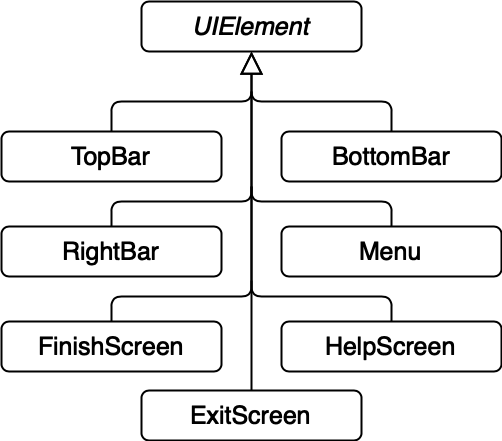
\includegraphics[scale=0.4]{resources/Typed_Objects_Diagram_UIElement_bb.png} 

    \end{figure}

\end{frame}

\begin{frame}
    \frametitle{Double Buffer}
    \begin{figure}
        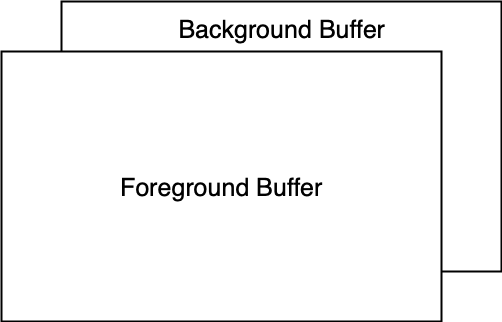
\includegraphics[scale=0.4]{resources/Double_buffer.png} 

    \end{figure}

\end{frame}


\subsection{Timeline}

\begin{frame}
    \frametitle{Timeline}
    \begin{figure}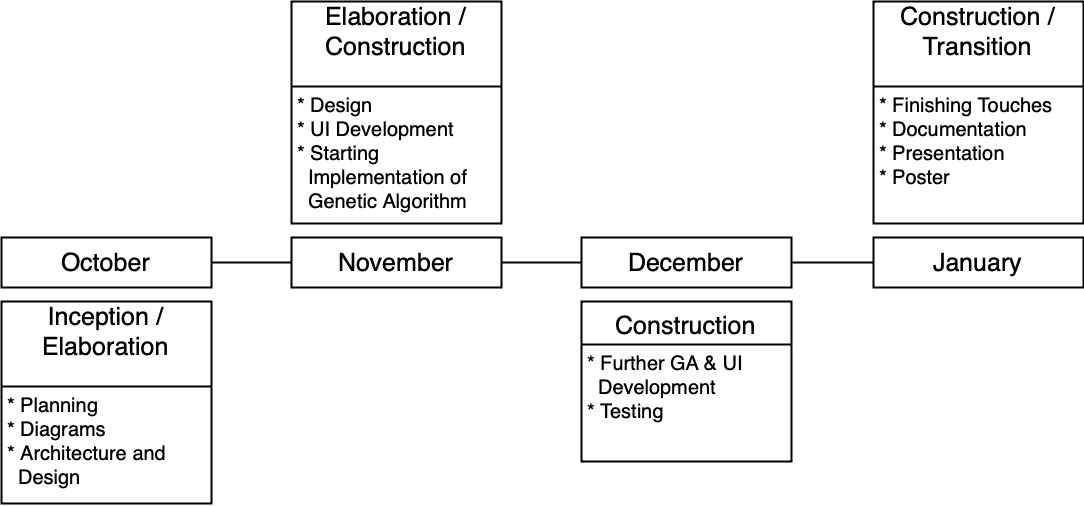
\includegraphics[scale=0.3]{resources/timeline.png} 

    \end{figure}

\end{frame}
\subsection{Future Work}
\begin{frame}
    \frametitle{Future Work}
    \begin{itemize}
        \item Score board
        \item Reuse of pretrained AI
        \item Reinforcement learning
        \item UI/UX improvements
    \end{itemize}

\end{frame}

\subsection{Lessons Learnt}
\begin{frame}
   \frametitle{Lessons Learnt}
   \begin{itemize}
       \item Managing project on Github (branching and merging)
       \item Importance of scrum meetings
       \item Proper time planning 
       \item Importance of communication
       \item Coherent task distribution 
       \item Adhering the coding standards (comments, diagrams etc.)
   \end{itemize}

\end{frame}
\begin{frame}
    \frametitle{}
    \centering
    \huge \textbf{Demo:}

\end{frame}

\end{document}
